\documentclass[conference]{IEEEtran}
\IEEEoverridecommandlockouts

\usepackage{cite}
\usepackage{amsmath,amssymb,amsfonts}
\usepackage{graphicx}
\usepackage{booktabs}
\usepackage{multirow}
\usepackage{xcolor}
\usepackage{url}
\usepackage{tikz}
\usetikzlibrary{arrows.meta,positioning,fit,calc,shapes.geometric}
\usepackage{pgfplots}
\pgfplotsset{compat=1.17}

\newcommand{\method}{TriSense-CenterPoint}
\newcommand{\vect}[1]{\mathbf{#1}}

\begin{document}

\title{\method: Lidar--Radar--Camera Fusion for Long-Range 3D Object Detection on Autonomous Trucks}

% For double-blind review, replace the block below with "Anonymous Authors".
\author{\IEEEauthorblockN{Author Name}
\IEEEauthorblockA{\textit{Department} \\
\textit{Affiliation}\\
City, Country \\
email@example.com}
}

\maketitle

\begin{abstract}
Autonomous trucks need to perceive objects at highway speeds and at ranges beyond those covered by most driving
benchmarks, around a vehicle whose size and articulated trailer create large blind regions for any single sensor.
We present \method, a bird's-eye-view (BEV) detector that fuses a merged six-lidar point cloud, six 4D imaging radars
and four cameras on the MAN TruckScenes dataset. The design starts from a voxel CenterPoint detector and adds a radar
pillar branch and a lift-splat camera branch through \emph{residual, zero-initialized} fusion blocks, so that the
fused network initially reproduces the lidar-only detector exactly and each new modality can only add information.
Radar Doppler measurements are ego-motion compensated with the truck's chassis velocity and yaw rate, kept
consistent under geometric data augmentation, and used directly as supervision through a Doppler consistency loss
on the predicted object velocity. The camera branch is supervised by lidar depth and a BEV heatmap, and a two-stage
schedule first warms up the new branches with the lidar detector frozen, then trains all components jointly with
modality dropout. Evaluated on the official TruckScenes test server, \method{} reaches \textbf{0.554~NDS} and
\textbf{0.505~mAP} under the challenge's sensor-history limits, with no test-time augmentation, future frames, maps
or external data. This is the highest NDS and mAP among the results published on the evaluation server at the time
of writing, ahead of the strongest lidar-only (0.551~NDS), camera--lidar (0.482) and radar--camera (0.420) entries. On the validation set it improves the lidar-only starting point from 0.433 to 0.548~NDS and lowers the
mean velocity error from 2.01 to 0.77~m/s. We also analyse the remaining failure modes per class and per driving
condition, which point to night, tunnels and fog as the open problems for truck perception.
\end{abstract}

\begin{IEEEkeywords}
3D object detection, sensor fusion, 4D radar, lidar, autonomous trucking, bird's-eye view
\end{IEEEkeywords}

% =====================================================================================================================
\section{Introduction}

Most progress in 3D object detection has been measured on passenger-car datasets such as KITTI~\cite{geiger2012kitti},
nuScenes~\cite{caesar2020nuscenes} and the Waymo Open Dataset~\cite{sun2020waymo}. Autonomous trucks pose a
different problem. A loaded semi-trailer truck needs a much longer distance to brake than a car, so the
detection range that matters is longer, and the MAN TruckScenes benchmark~\cite{fent2024truckscenes} therefore
evaluates vehicles up to 150~m away. The tractor and trailer occlude large parts of the scene for any single sensor,
which is why trucks carry many sensors around the cab. The operating domain is also broader: highways at high speed,
logistics terminals, rural roads, tunnels and bridges, in rain, fog and at night.

These conditions favour fusing complementary sensors. Lidar gives accurate geometry but its points become sparse at
long range and degrade in fog. Cameras give dense appearance and semantics but weak depth. 4D imaging radar is robust
to weather and lighting and measures radial velocity directly through the Doppler effect, but its point clouds are
sparse and noisy. Velocity matters in particular for trucks: at highway speeds, an error of a few m/s in an
object's velocity is a large error in where that object will be a second later.

In this paper we describe \method, the detector we submitted to the MAN TruckScenes 3D detection benchmark. It fuses
all three sensor types in a shared BEV grid on top of a strong lidar detector. Our contributions are:

\begin{itemize}
\item A tri-modal BEV detector for trucks that extends a voxel CenterPoint~\cite{yin2021centerpoint} with a radar
pillar branch and a lift-splat-shoot (LSS)~\cite{philion2020lss} camera branch through residual, zero-initialized
fusion blocks. The fused model starts out \emph{exactly} equal to the lidar detector, which makes training stable and
lets new modalities be added without degrading what the lidar model already does.
\item A physically consistent use of radar Doppler: ego-motion compensation with chassis velocity and yaw rate at
each radar's mount point, augmentations that transform the velocity vectors and lines of sight together with the
points, and a Doppler consistency loss that supervises the predicted object velocity with raw radial measurements.
\item A two-stage training recipe (frozen-detector warm-up of all new branches with auxiliary heads and lidar depth
supervision, followed by joint training with modality dropout).
\item Results on the official test server (0.554~NDS, 0.505~mAP), the highest among the published server results, with
a comparison against lidar-only, camera--lidar, radar--camera and radar-only entries and a per-class and per-condition
analysis that identifies where truck perception still fails.
\end{itemize}

% =====================================================================================================================
\section{Related Work}

\textbf{Lidar 3D detection.} VoxelNet~\cite{zhou2018voxelnet} learned features from voxelized point clouds, and
SECOND~\cite{yan2018second} made this practical with sparse 3D convolutions. PointPillars~\cite{lang2019pointpillars}
encodes vertical pillars for a purely 2D backbone. CenterPoint~\cite{yin2021centerpoint} represents objects as BEV
heatmap peaks and regresses their size, orientation and velocity, and together with class-balanced grouping and
sampling (CBGS)~\cite{zhu2019cbgs} is a strong baseline on nuScenes. We build on the voxel CenterPoint in
OpenPCDet~\cite{openpcdet2020}.

\textbf{Camera--lidar fusion in BEV.} LSS~\cite{philion2020lss} lifts image features into 3D with a per-pixel depth
distribution and splats them onto a BEV grid; BEVDet~\cite{huang2021bevdet} and BEVDepth~\cite{li2023bevdepth} turned
this into multi-camera detectors, the latter showing that explicit depth supervision from lidar is essential.
BEVFusion~\cite{liu2023bevfusion,liang2022bevfusion} fuses camera BEV features with lidar BEV features by
concatenation and convolution, while TransFusion~\cite{bai2022transfusion} fuses at the query level. Our camera
branch follows the BEVFusion style, but we fuse residually from a zero initialization and add an auxiliary camera
heatmap loss.

\textbf{Radar fusion.} CenterFusion~\cite{nabati2021centerfusion} associates radar points with camera detections,
and RadarNet~\cite{yang2020radarnet} fuses radar and lidar both early and late, using radial velocity to refine
object motion. CRN~\cite{kim2023crn} and RCBEVDet~\cite{lin2024rcbevdet} fuse radar and camera in BEV. 4D imaging
radar datasets such as View-of-Delft~\cite{palffy2022vod} showed the value of elevation and Doppler for road-user
detection. We use radar as a third modality next to lidar and cameras, and use its Doppler measurements both as an
input feature and as a training signal.

\textbf{Trucking datasets.} MAN TruckScenes~\cite{fent2024truckscenes} is the first large public dataset for
autonomous trucking. It provides six lidars, six 4D radars and four cameras, with annotations of 12 detection classes
including trailers, traffic signs and animals, and scene tags for weather, area, time of day, lighting and road
structure. Its benchmark uses nuScenes-style metrics with class-specific evaluation ranges of up to 150~m.

% =====================================================================================================================
\section{Dataset and Task}

TruckScenes scenes are 20~s long and annotated at 2~Hz keyframes. We use the official split: 20{,}907 training and
2{,}995 validation keyframes, and 5{,}960 test keyframes in 149 scenes, whose annotations are hidden behind an
evaluation server. Detections are scored with the official \texttt{truckscenes-devkit}: mean average precision (mAP)
over center-distance thresholds of 0.5, 1, 2 and 4~m, five true-positive (TP) errors for translation (mATE), scale
(mASE), orientation (mAOE), velocity (mAVE) and attributes (mAAE), and the nuScenes detection score
\begin{equation}
\mathrm{NDS} = \tfrac{1}{10}\Big[\,5\,\mathrm{mAP} + \textstyle\sum_{e \in \mathrm{TP}} \big(1 - \min(1, e)\big)\Big].
\end{equation}
Predictions and annotations are filtered by class-specific distance: 150~m for vehicles, 75~m for the other classes.

The benchmark limits the sensor history to about 0.5~s at inference: at most 6 past lidar sweeps, 11 past radar
sweeps and 6 past camera images. A submission may contain at most 500 boxes per keyframe, and it must declare which
sensors, maps, external data, future frames and test-time augmentation it used.

\textbf{Conversion to the nuScenes format.} To reuse mature nuScenes tooling, we convert TruckScenes into nuScenes
tables. The six lidars of every frame are merged into one virtual, ego-aligned top lidar. Each sensor's points are
transformed sensor $\rightarrow$ ego$(t_s)$ $\rightarrow$ global $\rightarrow$ ego$(t_\mathrm{ref})$ with the ego
poses at their own timestamps, which compensates the up to 50~ms firing offsets between the lidars. Radar and camera
data are read directly from the original dataset, together with their calibrations and ego poses. Evaluation always
runs against the original TruckScenes tables, so the scores are directly comparable to the leaderboard.

% =====================================================================================================================
\section{Method}

\begin{figure*}[t]
\centering
\resizebox{\textwidth}{!}{%
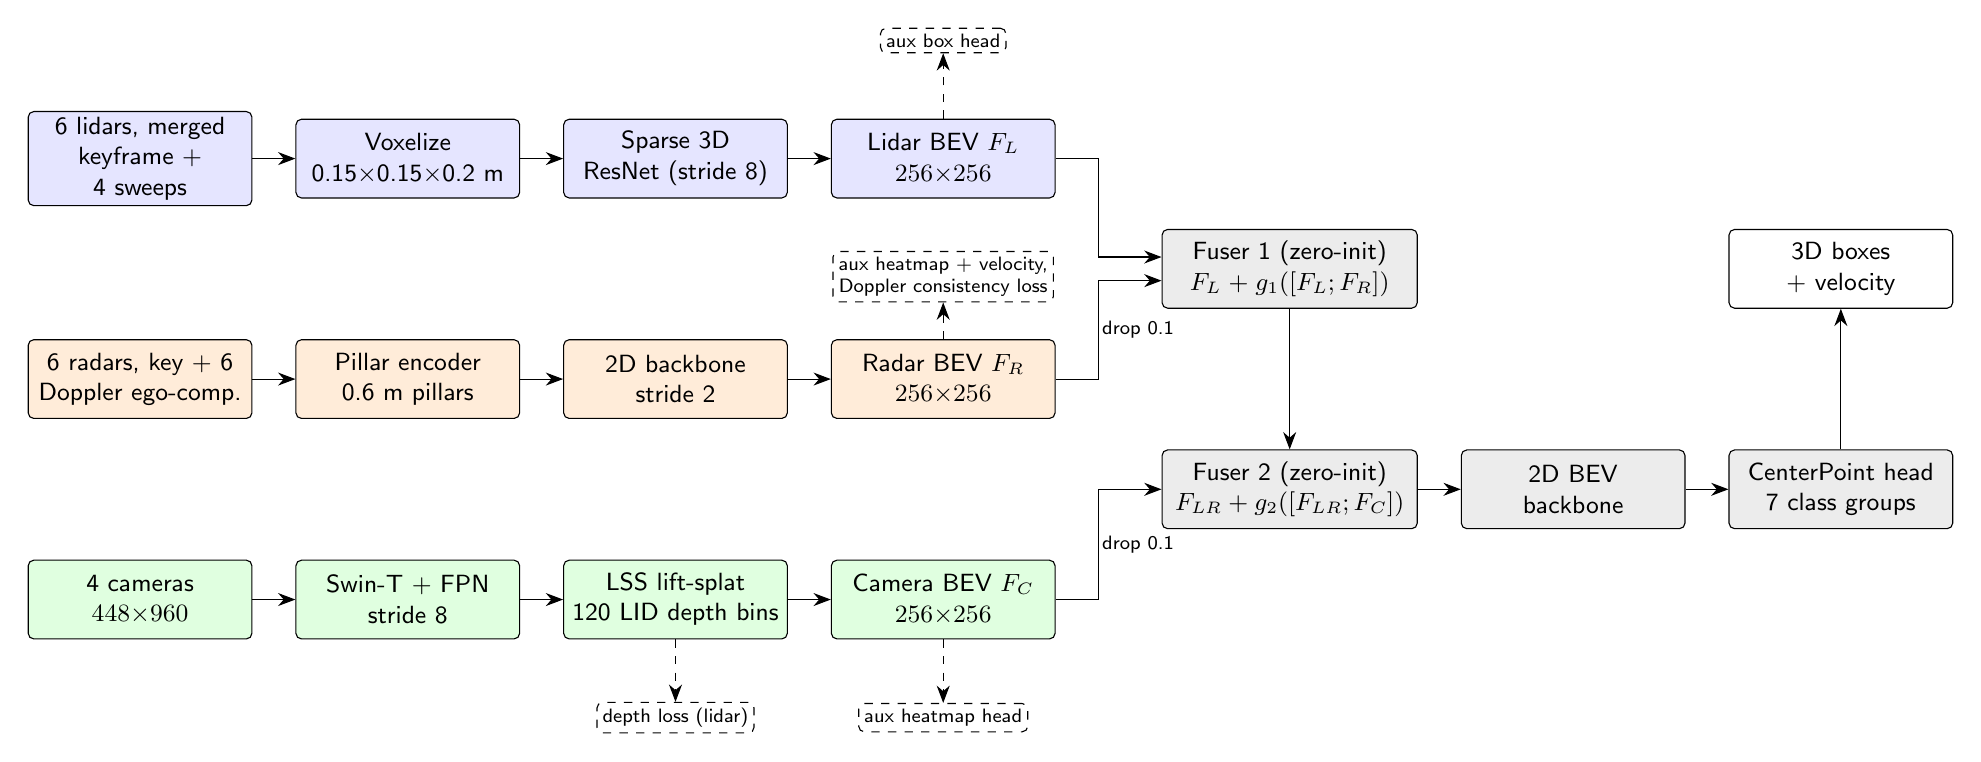
\begin{tikzpicture}[
  font=\sffamily\small,
  >={Stealth[length=2.2mm]},
  box/.style={draw, rounded corners=2pt, minimum height=10mm, text width=27mm, align=center, inner sep=2pt, fill=white},
  lidar/.style={box, fill=blue!10},
  radar/.style={box, fill=orange!15},
  cam/.style={box, fill=green!12},
  fuse/.style={box, fill=gray!15},
  aux/.style={draw, dashed, rounded corners=2pt, align=center, inner sep=2pt, font=\sffamily\scriptsize},
  lbl/.style={font=\sffamily\scriptsize, align=center, fill=white, inner sep=1pt}
]
% rows: lidar y=2.8, radar y=0, camera y=-2.8; columns x = 0, 2.7, 5.4, 8.1
\node[lidar] (lin)  at (0, 2.8) {6 lidars, merged\\keyframe + 4 sweeps};
\node[lidar] (lvox) at (3.4, 2.8) {Voxelize\\0.15$\times$0.15$\times$0.2 m};
\node[lidar] (l3d)  at (6.8, 2.8) {Sparse 3D\\ResNet (stride 8)};
\node[lidar] (lbev) at (10.2, 2.8) {Lidar BEV $F_L$\\$256{\times}256$};
\node[radar] (rin)  at (0, 0) {6 radars, key + 6\\Doppler ego-comp.};
\node[radar] (rvfe) at (3.4, 0) {Pillar encoder\\0.6 m pillars};
\node[radar] (rbb)  at (6.8, 0) {2D backbone\\stride 2};
\node[radar] (rbev) at (10.2, 0) {Radar BEV $F_R$\\$256{\times}256$};
\node[cam] (cin)  at (0, -2.8) {4 cameras\\$448{\times}960$};
\node[cam] (swin) at (3.4, -2.8) {Swin-T + FPN\\stride 8};
\node[cam] (lss)  at (6.8, -2.8) {LSS lift-splat\\120 LID depth bins};
\node[cam] (cbev) at (10.2, -2.8) {Camera BEV $F_C$\\$256{\times}256$};
\node[fuse, text width=31mm] (f1) at (14.6, 1.4) {Fuser 1 (zero-init)\\$F_L+g_1([F_L;F_R])$};
\node[fuse, text width=31mm] (f2) at (14.6, -1.4) {Fuser 2 (zero-init)\\$F_{LR}+g_2([F_{LR};F_C])$};
\node[fuse] (bb2d) at (18.2, -1.4) {2D BEV\\backbone};
\node[fuse] (head) at (21.6, -1.4) {CenterPoint head\\7 class groups};
\node[box]  (out)  at (21.6, 1.4) {3D boxes\\+ velocity};
% main flow
\foreach \u/\v in {lin/lvox, lvox/l3d, l3d/lbev, rin/rvfe, rvfe/rbb, rbb/rbev, cin/swin, swin/lss, lss/cbev}
  \draw[->] (\u) -- (\v);
\draw[->] (lbev.east) -- ++(0.55,0) |- ([yshift=1.5mm]f1.west);
\draw[->] (rbev.east) -- ++(0.55,0) |- node[lbl, pos=0.25, right] {drop 0.1} ([yshift=-1.5mm]f1.west);
\draw[->] (f1) -- (f2);
\draw[->] (cbev.east) -- ++(0.55,0) |- node[lbl, pos=0.25, right] {drop 0.1} (f2.west);
\draw[->] (f2) -- (bb2d);
\draw[->] (bb2d) -- (head);
\draw[->] (head) -- (out);
% training-only supervision
\node[aux] (alid) at (10.2, 4.3) {aux box head};
\node[aux] (arad) at (10.2, 1.3) {aux heatmap + velocity,\\Doppler consistency loss};
\node[aux] (acam) at (10.2, -4.3) {aux heatmap head};
\node[aux] (dep)  at (6.8, -4.3) {depth loss (lidar)};
\draw[->, dashed] (lbev) -- (alid);
\draw[->, dashed] (rbev) -- (arad);
\draw[->, dashed] (cbev) -- (acam);
\draw[->, dashed] (lss) -- (dep);
\end{tikzpicture}}
\caption{Overview of \method. Lidar, radar and camera features are built on the same $256{\times}256$ BEV grid with
1.2~m cells covering $\pm153.6$~m. Radar and camera BEV maps are added through residual fusers whose last
batch-norm scale is initialized to zero, so the network starts as the lidar-only CenterPoint. Dashed: losses used
only during training. Modality dropout zeroes the radar or camera BEV of a sample with probability 0.1.}
\label{fig:overview}
\end{figure*}

Fig.~\ref{fig:overview} gives an overview. Three branches produce BEV feature maps on a common grid: $256 \times
256$ cells of 1.2~m, covering $\pm153.6$~m around the truck, enough for the 150~m evaluation range. Two residual
fusers combine them, and a shared 2D backbone and CenterPoint head predict the boxes.

\subsection{Lidar Branch}

The merged lidar cloud of the keyframe and its 4 most recent past sweeps (well within the limit of 6) is voxelized
at $0.15 \times 0.15 \times 0.2$~m over $\pm153.6$~m horizontally and $[-4, 4]$~m vertically. Each point carries its
coordinates, intensity and time lag to the keyframe, and each voxel the mean of its points. A sparse 3D residual
backbone (VoxelResBackBone8x) with stride 8 yields the 256-channel lidar BEV map $F_L$ after height compression.
This branch and the detector head are those of a lidar-only CenterPoint trained on TruckScenes, which is also our
starting point.

\subsection{Radar Branch}

\textbf{Ego-motion compensation.} TruckScenes stores each radar return with its raw Doppler velocity, a vector
$\vect{v}^{\mathrm{rel}}$ along the line of sight in the sensor frame, which is not compensated for the truck's own
motion. A truck rotates noticeably while turning, and its radars are mounted metres away from the ego origin, so the
sensor's velocity differs from the chassis velocity. For a radar mounted at $\vect{t}_s$ in the ego frame with
rotation $R_s$, we compute the velocity of the mount point from the chassis velocity $\vect{v}_e$ and yaw rate
$\omega$,
\begin{equation}
\vect{v}_s = R_s^{\top}\big(\vect{v}_e + \omega\,\hat{\vect{z}} \times \vect{t}_s\big),
\end{equation}
and the compensated radial velocity of a return with unit ray $\hat{\vect{r}}$ (sensor frame) as
\begin{equation}
v_r = \vect{v}^{\mathrm{rel}} \cdot \hat{\vect{r}} + \vect{v}_s \cdot \hat{\vect{r}},
\end{equation}
which is zero for static objects. Each sample uses the keyframe and the 6 most recent past sweeps of each of the
6 radars (within the limit of 11). Their points are moved into the reference frame at the keyframe time using the
ego poses. Each point has the features $(x, y, z, \mathrm{RCS}, v_r \hat{r}_x, v_r \hat{r}_y, v_r, \Delta t)$, and we
also keep its ray and range for the augmentations and the Doppler loss.

\textbf{Equivariant augmentation.} The usual global flips, rotations and scalings of lidar detectors would make radar
velocities inconsistent with the scene if applied only to point positions. We apply each transform to the positions,
the radial velocity vectors and the rays together: flips negate the corresponding components, rotations rotate all
three, and scaling scales positions, ranges and velocities by the same factor as the box velocities.

\textbf{Encoder.} A PointPillars-style encoder~\cite{lang2019pointpillars} with 0.6~m pillars and 64 channels,
followed by a two-stage 2D backbone with stride 2, gives the radar BEV map $F_R$ on the lidar grid. The whole radar
branch has only 0.7~M parameters.

\subsection{Camera Branch}

The four cameras (left and right, front and back) have a resolution of $1980 \times 943$. Each image is resized by
0.485 and cropped to $448 \times 960$, mostly removing sky. An ImageNet-pretrained Swin-T~\cite{liu2021swin} backbone and an FPN~\cite{lin2017fpn} neck give 256-channel features at stride 8
($56 \times 120$). An LSS view transform~\cite{philion2020lss} predicts, for every feature cell, a categorical depth
distribution over $D = 120$ bins and an 80-channel context feature, and splats their outer product onto a 0.6~m BEV
grid that is pooled to the 1.2~m lidar grid. For a range of 150~m, uniform bins are either too coarse near the truck or
too many in total. We use linear-increasing discretization (LID)~\cite{reading2021caddn} instead, with bin edges
\begin{equation}
d_i = d_{\min} + (d_{\max} - d_{\min})\,\frac{i(i+1)}{D(D+1)}, \quad i = 0, \dots, D,
\end{equation}
with $d_{\min} = 1$~m and $d_{\max} = 153.6$~m. This gives bins of about 2~cm next to the truck and about 2.5~m
at the far end. The camera branch is camera-only: unlike some BEVFusion variants, lidar depth is never an input to
it, only a training target. The back cameras fire about 35~ms away from the lidar, so each camera-to-lidar transform
uses the ego pose at that camera's own timestamp.

\subsection{Residual Zero-Initialized Fusion}

Both fusion steps use the same block. Given a base BEV map $F_A$ and an added map $F_B$ on the same grid,
\begin{equation}
F' = F_A + g\big([F_A; F_B]\big),
\end{equation}
where $g$ is a $3{\times}3$ convolution, batch norm and ReLU to 256 channels, followed by a $3{\times}3$ convolution back
to the channels of $F_A$ and a batch norm whose scale $\gamma$ is initialized to zero. We first fuse radar into lidar,
$F_{LR} = F_L + g_1([F_L; F_R])$, and then the camera into the result,
$F_{LRC} = F_{LR} + g_2([F_{LR}; F_C])$. The shared 2D backbone and the CenterPoint head then work on $F_{LRC}$.

Because $\gamma = 0$, the fused network computes exactly the lidar detector when it is initialized from a lidar
checkpoint, whatever the random weights of the new branches. We verified this: after the warm-up stage, in which the
fusers are not trained, the model reproduces the lidar-only validation mAP to the fourth decimal
(Table~\ref{tab:val}). Training can therefore only move away from a good detector, rather than recover from the
noise that randomly initialized branches inject into the shared backbone.

\subsection{Detection Head and Auxiliary Supervision}

The detection head is the CenterPoint head~\cite{yin2021centerpoint}, with seven class groups: \{car\},
\{truck, other vehicle\}, \{bus, trailer\}, \{barrier\}, \{motorcycle, bicycle\}, \{pedestrian, traffic cone,
animal\} and \{traffic sign\}. It predicts a heatmap per class and regresses the center offset, height, size,
orientation and the 2D velocity. We train it with the focal heatmap loss and an $L_1$ regression loss
$\mathcal{L}_{\mathrm{det}}$.

Fusion alone gives a branch no direct reason to learn useful features, especially when the fused output starts out
ignoring it. We therefore add training-only auxiliary CenterPoint heads on each branch's BEV map \emph{before} fusion:
a full box head on $F_L$, a heatmap and velocity head on $F_R$, and a heatmap-only head on $F_C$. Camera BEV positions
are initially too coarse for box regression. None of these heads are run at inference.

\textbf{Doppler consistency loss.} Radar measures the projection of an object's velocity onto each line of sight. For
every ground-truth box $b$ with radar points $\mathcal{P}_b$ (inside the box enlarged by 1~m horizontally and 2~m
vertically), we take the velocity $\hat{\vect{v}}_b$ predicted by the radar auxiliary head at the BEV cell of the box
center, and penalize
\begin{equation}
\mathcal{L}_{\mathrm{Dop}} = \frac{1}{|\mathcal{B}|} \sum_{b \in \mathcal{B}} \frac{1}{|\mathcal{P}_b|}
\sum_{p \in \mathcal{P}_b} \mathrm{SmoothL1}\big(\hat{\vect{v}}_b \cdot \hat{\vect{r}}^{xy}_p - v_{r,p}\big),
\end{equation}
where $\mathcal{B}$ are the boxes with at least one radar point. The loss is averaged per box, so large trucks with
many returns do not dominate. This ties the predicted velocity to the actual measurements rather than only to
annotated velocities, which are derived from box positions in consecutive frames.

\textbf{Depth supervision.} Following BEVDepth~\cite{li2023bevdepth}, we project the current lidar sweep into each
augmented image and keep, for every stride-8 feature cell, the nearest lidar depth. Cells with lidar depth are
supervised with a binary cross-entropy between the predicted depth distribution and the one-hot depth bin. The total
loss is
\begin{equation}
\mathcal{L} = \mathcal{L}_{\mathrm{det}} + 0.5\big(\mathcal{L}^{L}_{\mathrm{aux}} + \mathcal{L}^{R}_{\mathrm{aux}}
 + \mathcal{L}^{C}_{\mathrm{aux}}\big) + 0.2\,\mathcal{L}_{\mathrm{Dop}} + 3\,\mathcal{L}_{\mathrm{depth}}.
\end{equation}

\subsection{Two-Stage Training}

\textbf{Lidar pre-training.} We first train the lidar-only CenterPoint with CBGS~\cite{zhu2019cbgs}, GT sampling and
global augmentations (batch 16, Adam~\cite{kingma2015adam} with a one-cycle schedule~\cite{smith2019superconvergence},
peak learning rate $5 \times 10^{-4}$). We use its checkpoint after 4 epochs.

\textbf{Stage A (warm-up).} All lidar modules, both fusers, the shared 2D backbone and the detection head are frozen,
with their batch-norm statistics fixed. Only the radar and camera branches and the three auxiliary heads train, on
the auxiliary, Doppler and depth losses, for one CBGS epoch (batch 8, peak learning rate $10^{-3}$). The fusers and the
detection head are not run, so the warm-up costs little memory, and the detector stays exactly the lidar detector.
Without this stage, freshly initialized auxiliary heads produce heatmap losses in the thousands in the first
iterations, and their gradients would reach the trained lidar backbone.

\textbf{Stage B (joint).} All parameters are trained with the full loss for 6 CBGS epochs (batch 6, one-cycle with
peak learning rate $7.5 \times 10^{-4}$, weight decay 0.01, gradient clipping at 10). With modality dropout, the radar
or camera BEV of each sample is zeroed with probability 0.1 before its fuser, so the detector does not depend on a
single added sensor. Lidar is never dropped, since every benchmark sample has lidar.

\textbf{Augmentation.} Stage B uses global flips along both axes, rotations in $\pm 45^\circ$, scaling in
$[0.9, 1.1]$ and translation noise ($\sigma = 0.5$~m), applied consistently to lidar, radar, boxes and the camera
extrinsics. Each image is also flipped, rotated in $\pm 5.4^\circ$ and randomly resized and cropped, with the exact
image-augmentation matrix kept for the view transform. We do not use GT sampling in the fused model, because pasted
lidar and radar objects would have no matching image content.

\textbf{Implementation.} The code is built on OpenPCDet~\cite{openpcdet2020} and trained with mixed precision on
NVIDIA A100 (80~GB) GPUs. The camera auxiliary head is kept in FP32, because its heatmap convolutions overflowed FP16
during the warm-up. The inference model (without auxiliary heads) has 44.5~M parameters, of which 27.5~M are in the
Swin-T backbone.

\subsection{Inference}

At test time the auxiliary heads, depth loss and modality dropout are disabled. The head keeps boxes with score above
0.1 and applies per-group NMS (IoU 0.2). We then keep the 500 highest-scoring boxes per keyframe over all groups,
because the benchmark rejects submissions with more. Attributes are assigned from the predicted velocity (moving if
faster than 0.2~m/s) and class, and classes without attributes (barrier, traffic cone) get none. No test-time
augmentation is used. Running the full pipeline, including data loading, on the 5{,}960 test keyframes takes about
37~minutes on one A100 with batch size 4.

% =====================================================================================================================
\section{Experiments}

\subsection{Test Set Results}


Our final model (stage B, epoch 6) was evaluated on the hidden test set under the benchmark's rules: inputs limited
to 4 past lidar sweeps, 6 past radar sweeps and the current camera images, and no maps, external data, future frames
or test-time augmentation. It reaches 0.505~mAP and 0.554~NDS (Table~\ref{tab:leaderboard}), slightly above its
validation scores (0.492~mAP, 0.548~NDS), so it does not appear overfitted to the validation set on which we selected
the checkpoint. The TP errors are similar on both splits: orientation error is lower on test (0.28 versus 0.38) and
velocity error is higher (0.87 versus 0.77~m/s).

\subsection{Comparison with Other Methods}

\begin{table*}[t]
\centering
\caption{Comparison on the TruckScenes test set. All entries are results published on the official evaluation server
(accessed November~2, 2026), with the sensors each submission declared. For methods with several submissions we
list the best one; debugging and dummy submissions are omitted. L: lidar, R: radar, C: camera. $\dagger$: declared use of
external data. Lower is better for the TP errors.}
\label{tab:leaderboard}
\setlength{\tabcolsep}{5pt}
\begin{tabular}{llccc|cc|ccccc}
\toprule
\# & Method & L & R & C & NDS$\uparrow$ & mAP$\uparrow$ & mATE & mASE & mAOE & mAVE & mAAE \\
\midrule
1 & \textbf{\method{} (ours)}                     & \checkmark & \checkmark & \checkmark & \textbf{0.554} & \textbf{0.505} & \textbf{0.373} & 0.359 & \textbf{0.276} & 0.868 & 0.108 \\
2 & Unnamed submission (Aug.\ 2026)                & \checkmark &            &            & 0.551 & 0.481 & 0.377 & 0.373 & 0.293 & \textbf{0.763} & \textbf{0.088} \\
3 & Unnamed submission (Mar.\ 2026)                & \checkmark &            & \checkmark & 0.482 & 0.485 & 0.428 & 0.381 & 0.542 & 2.240 & 0.255 \\
4 & SpaRC~\cite{wolters2024sparc}                  &            & \checkmark & \checkmark & 0.420 & 0.332 & 0.717 & 0.393 & 0.355 & 0.784 & 0.208 \\
5 & CenterPoint~\cite{yin2021centerpoint}          & \checkmark &            &            & 0.410 & 0.267 & 0.409 & \textbf{0.352} & 0.277 & 2.730 & 0.201 \\
6 & RaGSplat                                       &            & \checkmark &            & 0.236 & 0.161 & 0.680 & 0.697 & 0.594 & 0.897 & 0.573 \\
7 & HyDRa$^\dagger$~\cite{wolters2024hydra}        &            & \checkmark & \checkmark & 0.224 & 0.128 & 0.725 & 0.544 & 0.744 & 1.180 & 0.388 \\
8 & DRaGAN                                         &            & \checkmark &            & 0.209 & 0.088 & 0.728 & 0.639 & 0.644 & 1.044 & 0.339 \\
9 & PETR~\cite{liu2022petr}$^\ast$                 &            &            & \checkmark & 0.121 & 0.022 & 1.125 & 0.686 & 0.647 & 1.499 & 0.564 \\
10 & RadarGNN~\cite{fent2023radargnn}              &            & \checkmark &            & 0.108 & 0.070 & 0.892 & 0.809 & 1.132 & 8.003 & 0.571 \\
\bottomrule
\multicolumn{12}{l}{\footnotesize $^\ast$PETR is a camera-only method; its submission declared lidar instead of camera input.}
\end{tabular}
\end{table*}

\begin{table}[t]
\centering
\caption{Test AP per class of the strongest entries of Table~\ref{tab:leaderboard}. \#2: unnamed lidar-only, \#3:
unnamed camera--lidar submission.}
\label{tab:lbclass}
\setlength{\tabcolsep}{3.5pt}
\begin{tabular}{lccccc}
\toprule
Class & Ours & \#2 (L) & \#3 (L+C) & SpaRC & CenterPoint \\
\midrule
Car           & 0.842 & \textbf{0.871} & 0.822 & 0.581 & 0.329 \\
Truck         & 0.588 & 0.587 & \textbf{0.591} & 0.392 & 0.227 \\
Bus           & \textbf{0.401} & 0.190 & 0.372 & 0.148 & 0.055 \\
Trailer       & 0.652 & \textbf{0.665} & 0.647 & 0.494 & 0.336 \\
Other vehicle & \textbf{0.254} & 0.002 & 0.024 & 0.089 & 0.138 \\
Pedestrian    & 0.584 & \textbf{0.674} & 0.579 & 0.279 & 0.451 \\
Motorcycle    & 0.598 & \textbf{0.620} & 0.576 & 0.373 & 0.222 \\
Bicycle       & 0.136 & 0.165 & \textbf{0.256} & 0.222 & 0.064 \\
Traffic cone  & 0.720 & \textbf{0.781} & 0.758 & 0.553 & 0.547 \\
Barrier       & \textbf{0.565} & 0.443 & 0.451 & 0.347 & 0.415 \\
Animal        & 0.000 & 0.000 & 0.000 & 0.000 & 0.000 \\
Traffic sign  & 0.719 & \textbf{0.770} & 0.745 & 0.510 & 0.423 \\
\bottomrule
\end{tabular}
\end{table}

Table~\ref{tab:leaderboard} compares \method{} with all methods whose results are published on the evaluation server.
It has the highest NDS and mAP, and the lowest translation and orientation errors. Three groups of entries
stand out.

\textbf{Lidar-based methods.} The strongest other entry is an unnamed lidar-only submission (0.551~NDS). Our NDS
margin over it is small (+0.003), but our mAP is 2.4 points higher. Table~\ref{tab:lbclass} shows that the two
models have different strengths. \method{} is far better on the rare and large classes: other vehicles
(0.254 versus 0.002~AP), buses (0.401 versus 0.190) and barriers (0.565 versus 0.443). The lidar-only model is better on
the small, frequent classes (pedestrians, traffic cones, signs) and on cars, and its velocity error is lower (0.76
versus 0.87~m/s). This suggests that a better-tuned lidar branch, for example with longer training or GT sampling,
could be combined with our fusion to gain on both sides. Compared with the CenterPoint entry, which uses the same
detector family with lidar only, our model scores 0.145 higher NDS and 0.238 higher mAP. Part of this gap is due to
training and tuning, not only to fusion.

\textbf{Camera--lidar fusion.} The best camera--lidar entry has a similar mAP (0.485) but a much lower NDS (0.482),
because its velocity (2.24~m/s) and orientation (0.54~rad) errors are large. Our model lowers the velocity error by 61\% and
roughly halves the orientation error, which is consistent with radar Doppler adding the motion information that neither lidar nor cameras measure
directly.

\textbf{Radar--camera and radar-only methods.} Without lidar, the best method, SpaRC~\cite{wolters2024sparc}, reaches
0.420~NDS. Its velocity error (0.78~m/s) is close to ours, which confirms the value of radar for motion. However, its
translation error is almost twice ours (0.72 versus 0.37~m), the expected cost of missing lidar geometry at long
range. Radar-only methods stay below 0.24~NDS. This shows that radar cannot replace lidar for long-range truck
perception, but it is a valuable addition to it.

\subsection{Effect of Fusion and Training Progress}

\begin{table}[t]
\centering
\caption{Validation results. The lidar row is the starting checkpoint of both stages. Stage A must equal it, since the
zero-initialized fusers are not trained in stage A.}
\label{tab:val}
\setlength{\tabcolsep}{3.2pt}
\begin{tabular}{lcccccc}
\toprule
Model & mAP$\uparrow$ & NDS$\uparrow$ & mATE & mASE & mAOE & mAVE \\
\midrule
Lidar CenterPoint (ep.\ 4)   & 0.334 & 0.433 & 0.430 & 0.327 & 0.461 & 2.011 \\
+ Stage A (warm-up)          & 0.334 & 0.433 & 0.429 & 0.327 & 0.469 & 2.011 \\
\midrule
Stage B, epoch 2             & 0.417 & 0.466 & 0.460 & 0.400 & 0.443 & 1.630 \\
Stage B, epoch 3             & 0.482 & 0.504 & 0.429 & 0.400 & 0.424 & 1.281 \\
Stage B, epoch 4             & 0.472 & 0.505 & 0.394 & 0.388 & 0.424 & 1.060 \\
Stage B, epoch 5             & \textbf{0.497} & 0.545 & 0.359 & 0.374 & 0.380 & 0.823 \\
Stage B, epoch 6 (final)     & 0.492 & \textbf{0.548} & \textbf{0.358} & 0.380 & \textbf{0.377} & \textbf{0.774} \\
\bottomrule
\end{tabular}
\end{table}

\begin{figure}[t]
\centering
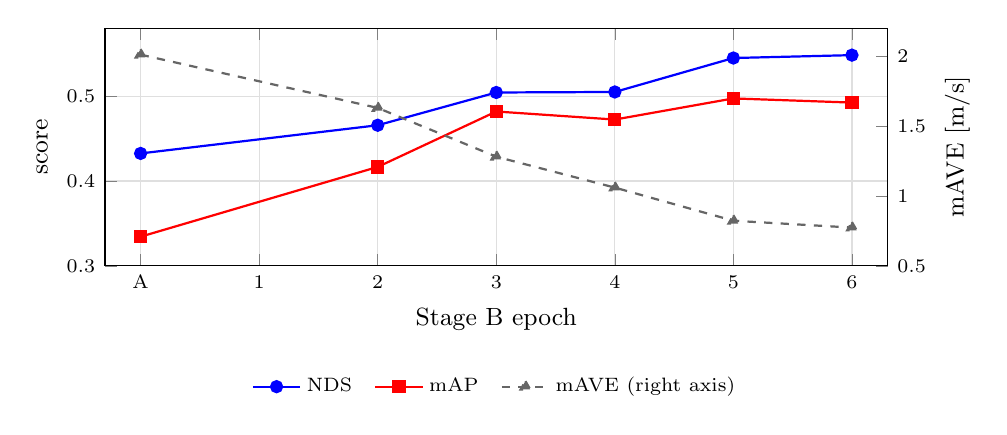
\begin{tikzpicture}
\begin{axis}[
  width=0.95\columnwidth, height=4.6cm,
  xlabel={Stage B epoch}, ylabel={score},
  xmin=-0.3, xmax=6.3, ymin=0.30, ymax=0.58,
  xtick={0,1,2,3,4,5,6}, xticklabels={A,1,2,3,4,5,6},
  legend style={at={(0.5,-0.42)}, anchor=north, legend columns=3, font=\scriptsize, draw=none, /tikz/every even column/.append style={column sep=6pt}},
  grid=major, grid style={gray!25}, tick label style={font=\scriptsize}, label style={font=\small},
  axis y line*=left
]
\addplot[blue, mark=*, thick] coordinates {(0,0.4325) (2,0.4657) (3,0.5043) (4,0.5049) (5,0.5449) (6,0.5483)};
\addlegendentry{NDS}
\addplot[red, mark=square*, thick] coordinates {(0,0.3344) (2,0.4166) (3,0.4819) (4,0.4724) (5,0.4973) (6,0.4924)};
\addlegendentry{mAP}
\addlegendimage{black!60, dashed, mark=triangle*, thick}\addlegendentry{mAVE (right axis)}
\end{axis}
\begin{axis}[
  width=0.95\columnwidth, height=4.6cm,
  xmin=-0.3, xmax=6.3, ymin=0.5, ymax=2.2,
  axis y line*=right, axis x line=none, ylabel={mAVE [m/s]},
  tick label style={font=\scriptsize}, label style={font=\small}
]
\addplot[black!60, dashed, mark=triangle*, thick] coordinates {(0,2.011) (2,1.630) (3,1.281) (4,1.060) (5,0.823) (6,0.774)};
\end{axis}
\end{tikzpicture}
\caption{Validation NDS, mAP and velocity error over training. ``A'' is the model after the warm-up stage, which
equals the lidar-only starting point. Epoch 1 was not evaluated.}
\label{fig:curve}
\end{figure}

Table~\ref{tab:val} and Fig.~\ref{fig:curve} follow the model through training on the validation set. After the
warm-up, the network is still the lidar detector (0.334~mAP, 0.433~NDS), as intended. Joint training then raises mAP by
0.158 and NDS by 0.115. The largest single improvement is in velocity: mAVE falls steadily from 2.01 to 0.77~m/s,
a 62\% reduction, while translation and orientation errors fall by 17\% and 18\%. Scale error rises from 0.33 to
0.38. We attribute this to the dropped GT sampling, which removes the many pasted, well-sampled objects that the lidar
model saw in training. The two last epochs have nearly the same scores, so we submitted the last one, which has the best
NDS and the lowest TP errors.

\textbf{Caveat on attribution.} These gains combine the effect of the added sensors with that of seven further
epochs of training, the last six with a fully annealed learning rate, while the lidar checkpoint was taken early in a
20-epoch schedule. They therefore give an upper bound on the contribution of fusion, not a controlled ablation. The
size and direction of some changes still point to the added modalities. The velocity error, which radar measures
directly and our Doppler loss supervises, falls the most. The classes that gain most are those that lidar sees with
few points at long range (bus: 0.12$\rightarrow$0.42~AP, motorcycle: 0.10$\rightarrow$0.65, bicycle:
0.10$\rightarrow$0.44, Table~\ref{tab:class}). We discuss the missing ablations in Section~\ref{sec:limits}.

\subsection{Per-Class Results}

\begin{table}[t]
\centering
\caption{AP per class (mean over distance thresholds). Lidar: starting checkpoint on validation; Ours: final model.}
\label{tab:class}
\setlength{\tabcolsep}{4pt}
\begin{tabular}{lccc}
\toprule
Class & Lidar (val) & Ours (val) & Ours (test) \\
\midrule
Car            & 0.760 & 0.830 & 0.842 \\
Truck          & 0.473 & 0.588 & 0.588 \\
Bus            & 0.124 & 0.423 & 0.401 \\
Trailer        & 0.545 & 0.667 & 0.652 \\
Other vehicle  & 0.101 & 0.197 & 0.254 \\
Pedestrian     & 0.512 & 0.584 & 0.584 \\
Motorcycle     & 0.103 & 0.647 & 0.598 \\
Bicycle        & 0.095 & 0.444 & 0.136 \\
Traffic cone   & 0.574 & 0.729 & 0.720 \\
Barrier        & 0.139 & 0.111 & 0.565 \\
Animal         & 0.000 & 0.000 & 0.000 \\
Traffic sign   & 0.586 & 0.687 & 0.719 \\
\midrule
mAP            & 0.334 & 0.492 & 0.505 \\
\bottomrule
\end{tabular}
\end{table}

Table~\ref{tab:class} breaks AP down by class. On validation, the fused model improves every class except barrier
(0.139$\rightarrow$0.111) and animal, which no model detects. Large vehicles benefit strongly: cars, trucks and
trailers gain 7--12 AP points, and buses more than triple their AP. 

Classes with few validation instances are very sensitive to the evaluated split and checkpoint. Barrier AP is 0.11
on validation but 0.57 on test, and bicycle AP is 0.44 on validation but 0.14 on test. Even for the lidar model
alone, motorcycle AP moved from 0.40 at epoch 3 to 0.10 at epoch 4 of the same run. Results for these classes should
be read as noisy, and the mean over 12 classes is noticeably affected by them. The animal class, with only a handful of
annotations, remains at zero AP. It would need targeted resampling or a dedicated head.

\subsection{Performance under Driving Conditions}

\begin{table}[t]
\centering
\caption{Test NDS / mAP per scene tag, as reported by the evaluation server. Conditions absent from the test set
(snow, hail, spring, parking areas) are omitted.}
\label{tab:cond}
\setlength{\tabcolsep}{3pt}
\begin{tabular}{llcc|llcc}
\toprule
& Tag & NDS & mAP & & Tag & NDS & mAP \\
\midrule
\multirow{4}{*}{\rotatebox{90}{Weather}} & clear    & 0.534 & 0.486 & \multirow{4}{*}{\rotatebox{90}{Lighting}} & illuminated & 0.553 & 0.509 \\
 & overcast & 0.510 & 0.445 & & twilight & 0.342 & 0.280 \\
 & rain     & 0.426 & 0.419 & & dark     & 0.332 & 0.269 \\
 & fog      & 0.275 & 0.281 & & glare    & 0.294 & 0.277 \\
\midrule
\multirow{5}{*}{\rotatebox{90}{Area}} & highway  & 0.472 & 0.441 & \multirow{4}{*}{\rotatebox{90}{Structure}} & regular & 0.560 & 0.527 \\
 & terminal    & 0.415 & 0.405 & & bridge    & 0.467 & 0.374 \\
 & rural       & 0.395 & 0.411 & & underpass & 0.426 & 0.395 \\
 & city        & 0.378 & 0.287 & & tunnel    & 0.220 & 0.210 \\
 & residential & 0.368 & 0.267 & & & & \\
\midrule
\multirow{4}{*}{\rotatebox{90}{Daytime}} & morning & 0.543 & 0.476 & \multirow{3}{*}{\rotatebox{90}{Season}} & summer & 0.582 & 0.577 \\
 & noon    & 0.541 & 0.500 & & winter & 0.473 & 0.425 \\
 & evening & 0.331 & 0.287 & & autumn & 0.443 & 0.366 \\
 & night   & 0.000 & 0.000 & & & & \\
\midrule
\multicolumn{4}{l|}{Roadworks: 0.369 / 0.388} & \multicolumn{4}{l}{No roadworks: 0.546 / 0.493} \\
\bottomrule
\end{tabular}
\end{table}

The test server also reports scores per scene tag (Table~\ref{tab:cond}). Each tag subset is evaluated on its own,
with its own class mix, so a subset can score lower than the full test set even if every subset is detected
equally well. With that caveat, the breakdown shows clear trends:

\begin{itemize}
\item \textbf{Lighting and time of day} matter most. Twilight, dark and glare scenes score 0.29--0.34~NDS against
0.55 in illuminated scenes, and the night subset scores zero. Since lidar and radar do not depend on light, the zero
on night scenes more likely reflects a very small or unusual subset (for example, only rare classes) than a complete
failure of the detector, but it shows that the camera branch, trained on few dark images, contributes little there.
\item \textbf{Fog} (0.28~NDS) is the hardest weather condition, consistent with lidar's sensitivity to fog. It
suggests that the radar branch is not yet weighted strongly enough when lidar degrades. Modality dropout of
\emph{lidar} features, which we did not use, may help.
\item \textbf{Tunnels} (0.22~NDS) are the hardest road structure. They combine poor lighting with enclosing walls,
which plausibly cause radar multipath reflections and clutter in the lidar data; the tunnel subset is also small.
Bridges and underpasses are less affected.
\item \textbf{Urban scenes} (city, residential: 0.37~NDS) are harder than highways (0.47). They contain more
pedestrians, cyclists and occlusions, while highway scenes are dominated by vehicles, which the model detects best.
\end{itemize}

\subsection{Discussion: Velocity Estimation}

Velocity remains the largest TP error (0.87~m/s on test). Object speeds on highways are high, our lidar history is
short (0.4~s), and annotated velocities are finite differences of box positions, which makes them noisy. Doppler is
the most direct velocity signal, but our model applies the Doppler loss only to the radar branch. Applying it to the
fused head is a natural next step.

\subsection{Limitations}
\label{sec:limits}

Our study has several limitations. (i)~As discussed above, we do not have controlled ablations. The comparison with
the lidar model mixes fusion with additional training, and we did not train lidar+radar or lidar+camera variants
with the same schedule. The individual contributions of the Doppler loss, the depth loss, the auxiliary heads and
modality dropout are therefore not isolated. (ii)~All numbers come from a single training run, so we cannot give
variance estimates, which matter for the rare classes. (iii)~Images are processed at about half resolution, which
limits long-range camera detections. (iv)~The fused model does not use GT sampling, which costs scale accuracy and
may cost recall on rare classes. A multi-modal GT sampler that also pastes image patches could recover both.

% =====================================================================================================================
\section{Conclusion}

We presented \method, a lidar--radar--camera BEV detector for autonomous trucks. Residual, zero-initialized fusion
lets radar and camera branches be added to a trained lidar detector without ever degrading it. A physically
consistent treatment of radar Doppler, from ego-motion compensation to a Doppler consistency loss, supports
velocity estimation, and a two-stage training recipe keeps the joint training stable. On the MAN TruckScenes test set,
the model reaches 0.554~NDS and 0.505~mAP under the benchmark's sensor-history limits, the best result published on the
evaluation server, with the largest margins on rare vehicle classes and on velocity and orientation compared with
camera--lidar fusion. The per-condition analysis
shows that night, glare, fog and tunnels are still far from solved. Making the detector shift its weight towards
radar when light or visibility degrades is, in our view, the most important direction for future work on truck
perception.

\section*{Acknowledgment}
% Add funding / compute acknowledgments here.
We thank the MAN TruckScenes team for releasing the dataset and maintaining the evaluation server.

\bibliographystyle{IEEEtran}
\bibliography{refs}

\end{document}
